\section{Wm4::Matrix3$<$ Real $>$ Class Template Reference}
\label{classWm4_1_1Matrix3}\index{Wm4::Matrix3@{Wm4::Matrix3}}
{\tt \#include $<$Wm4Matrix3.h$>$}

Collaboration diagram for Wm4::Matrix3$<$ Real $>$:\begin{figure}[H]
\begin{center}
\leavevmode
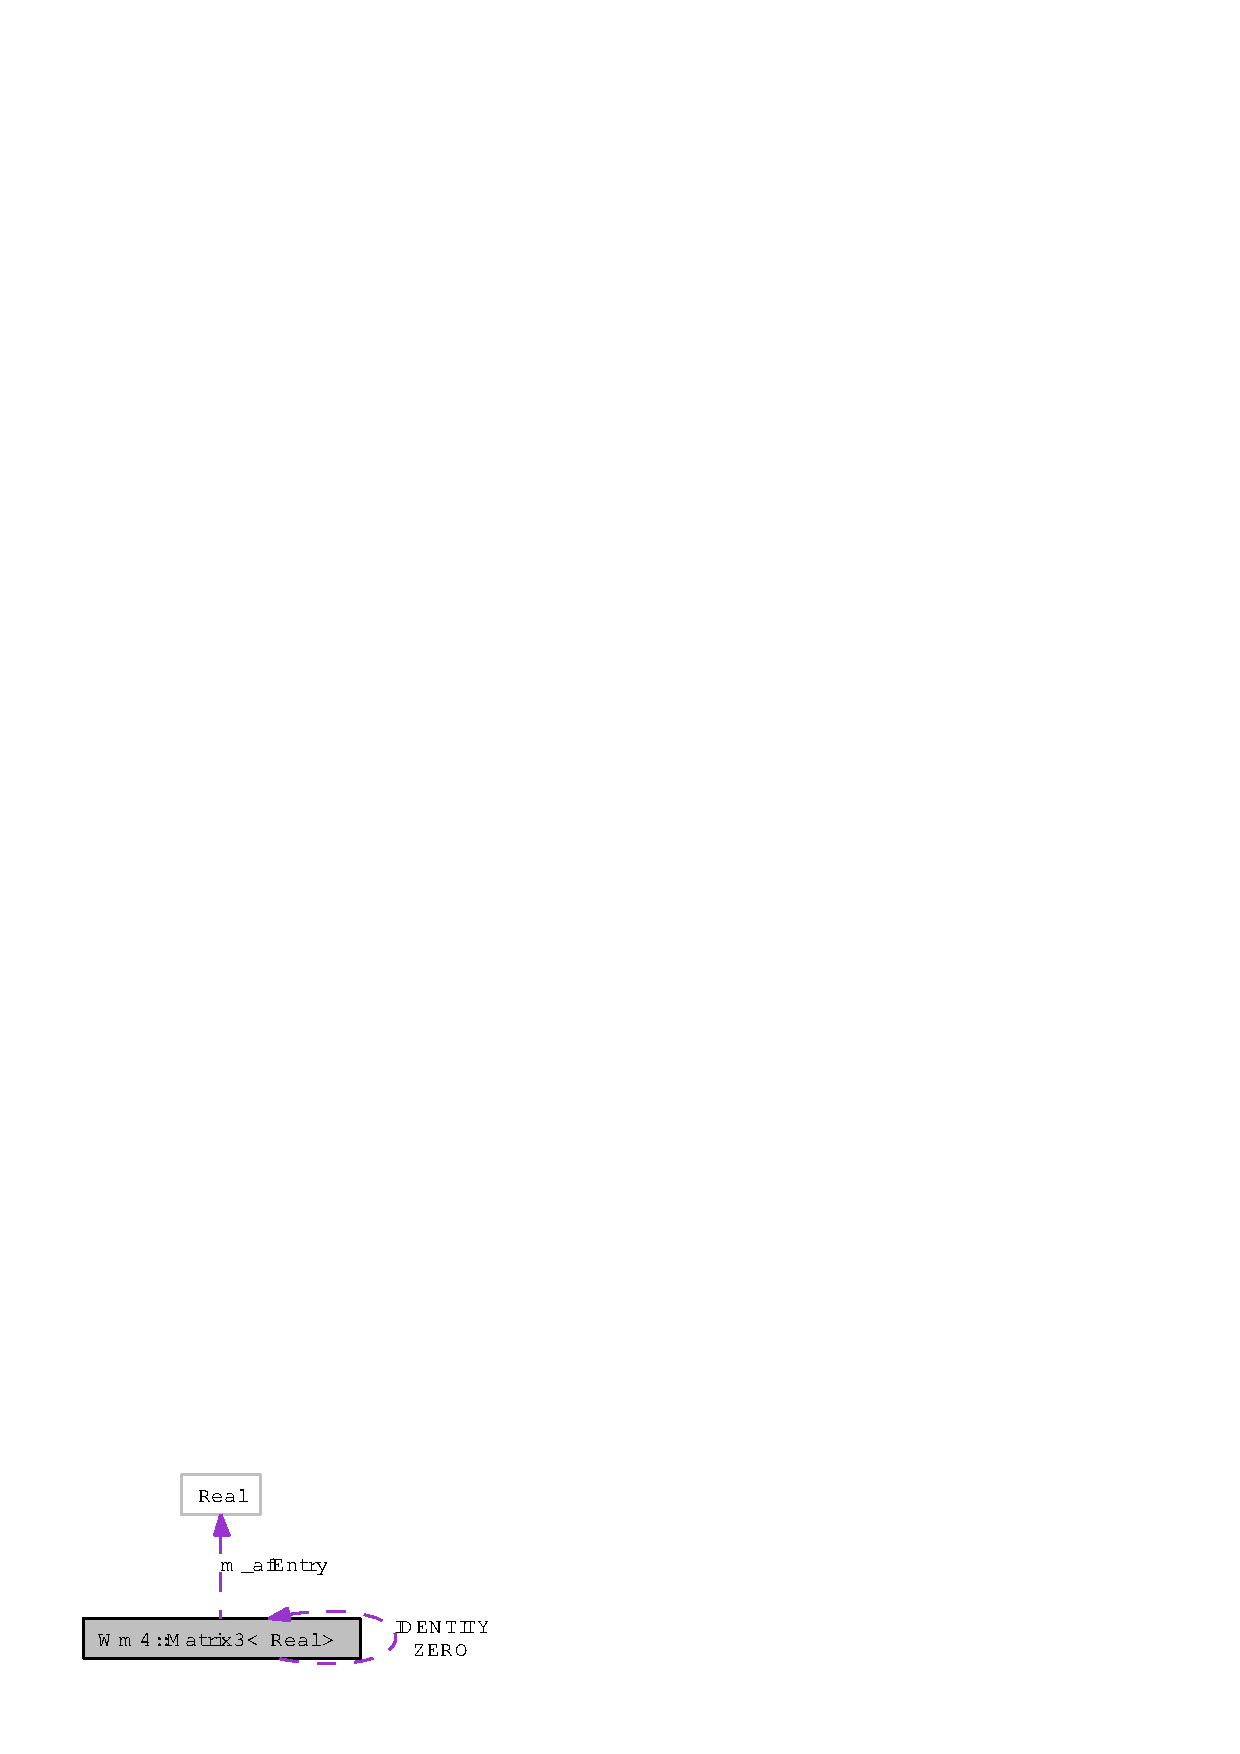
\includegraphics[width=120pt]{classWm4_1_1Matrix3__coll__graph}
\end{center}
\end{figure}
\subsection*{Public Types}
\begin{CompactItemize}
\item 
enum {\bf Euler\-Result} \{ {\bf EA\_\-UNIQUE}, 
{\bf EA\_\-NOT\_\-UNIQUE\_\-SUM}, 
{\bf EA\_\-NOT\_\-UNIQUE\_\-DIF}
 \}
\end{CompactItemize}
\subsection*{Public Member Functions}
\begin{CompactItemize}
\item 
{\bf Matrix3} (bool b\-Zero=true)
\item 
{\bf Matrix3} (const {\bf Matrix3} \&rk\-M)
\item 
{\bf Matrix3} (Real f\-M00, Real f\-M01, Real f\-M02, Real f\-M10, Real f\-M11, Real f\-M12, Real f\-M20, Real f\-M21, Real f\-M22)
\item 
{\bf Matrix3} (const Real af\-Entry[9], bool b\-Row\-Major)
\item 
{\bf Matrix3} (const {\bf Vector3}$<$ Real $>$ \&rk\-U, const {\bf Vector3}$<$ Real $>$ \&rk\-V, const {\bf Vector3}$<$ Real $>$ \&rk\-W, bool b\-Columns)
\item 
{\bf Matrix3} (const {\bf Vector3}$<$ Real $>$ $\ast$ak\-V, bool b\-Columns)
\item 
{\bf Matrix3} (Real f\-M00, Real f\-M11, Real f\-M22)
\item 
{\bf Matrix3} (const {\bf Vector3}$<$ Real $>$ \&rk\-Axis, Real f\-Angle)
\item 
{\bf Matrix3} (const {\bf Vector3}$<$ Real $>$ \&rk\-U, const {\bf Vector3}$<$ Real $>$ \&rk\-V)
\item 
{\bf Matrix3} \& {\bf Make\-Zero} ()
\item 
{\bf Matrix3} \& {\bf Make\-Identity} ()
\item 
{\bf Matrix3} \& {\bf Make\-Diagonal} (Real f\-M00, Real f\-M11, Real f\-M22)
\item 
{\bf Matrix3} \& {\bf From\-Axis\-Angle} (const {\bf Vector3}$<$ Real $>$ \&rk\-Axis, Real f\-Angle)
\item 
{\bf Matrix3} \& {\bf Make\-Tensor\-Product} (const {\bf Vector3}$<$ Real $>$ \&rk\-U, const {\bf Vector3}$<$ Real $>$ \&rk\-V)
\item 
{\bf operator const Real $\ast$} () const
\item 
{\bf operator Real $\ast$} ()
\item 
const Real $\ast$ {\bf operator[$\,$]} (int i\-Row) const
\item 
Real $\ast$ {\bf operator[$\,$]} (int i\-Row)
\item 
Real {\bf operator()} (int i\-Row, int i\-Col) const
\item 
Real \& {\bf operator()} (int i\-Row, int i\-Col)
\item 
void {\bf Set\-Row} (int i\-Row, const {\bf Vector3}$<$ Real $>$ \&rk\-V)
\item 
{\bf Vector3}$<$ Real $>$ {\bf Get\-Row} (int i\-Row) const
\item 
void {\bf Set\-Column} (int i\-Col, const {\bf Vector3}$<$ Real $>$ \&rk\-V)
\item 
{\bf Vector3}$<$ Real $>$ {\bf Get\-Column} (int i\-Col) const
\item 
void {\bf Get\-Column\-Major} (Real $\ast$af\-CMajor) const
\item 
{\bf Matrix3} \& {\bf operator=} (const {\bf Matrix3} \&rk\-M)
\item 
bool {\bf operator==} (const {\bf Matrix3} \&rk\-M) const
\item 
bool {\bf operator!=} (const {\bf Matrix3} \&rk\-M) const
\item 
bool {\bf operator$<$} (const {\bf Matrix3} \&rk\-M) const
\item 
bool {\bf operator$<$=} (const {\bf Matrix3} \&rk\-M) const
\item 
bool {\bf operator$>$} (const {\bf Matrix3} \&rk\-M) const
\item 
bool {\bf operator$>$=} (const {\bf Matrix3} \&rk\-M) const
\item 
{\bf Matrix3} {\bf operator+} (const {\bf Matrix3} \&rk\-M) const
\item 
{\bf Matrix3} {\bf operator-} (const {\bf Matrix3} \&rk\-M) const
\item 
{\bf Matrix3} {\bf operator $\ast$} (const {\bf Matrix3} \&rk\-M) const
\item 
{\bf Matrix3} {\bf operator $\ast$} (Real f\-Scalar) const 
\item 
{\bf Matrix3} {\bf operator/} (Real f\-Scalar) const 
\item 
{\bf Matrix3} {\bf operator-} () const
\item 
{\bf Matrix3} \& {\bf operator+=} (const {\bf Matrix3} \&rk\-M)
\item 
{\bf Matrix3} \& {\bf operator-=} (const {\bf Matrix3} \&rk\-M)
\item 
{\bf Matrix3} \& {\bf operator $\ast$=} (Real f\-Scalar)
\item 
{\bf Matrix3} \& {\bf operator/=} (Real f\-Scalar)
\item 
{\bf Vector3}$<$ Real $>$ {\bf operator $\ast$} (const {\bf Vector3}$<$ Real $>$ \&rk\-V) const
\item 
{\bf Matrix3} {\bf Transpose} () const
\item 
{\bf Matrix3} {\bf Transpose\-Times} (const {\bf Matrix3} \&rk\-M) const
\item 
{\bf Matrix3} {\bf Times\-Transpose} (const {\bf Matrix3} \&rk\-M) const
\item 
{\bf Matrix3} {\bf Inverse} () const
\item 
{\bf Matrix3} {\bf Adjoint} () const
\item 
Real {\bf Determinant} () const
\item 
Real {\bf QForm} (const {\bf Vector3}$<$ Real $>$ \&rk\-U, const {\bf Vector3}$<$ Real $>$ \&rk\-V) const
\item 
{\bf Matrix3} {\bf Times\-Diagonal} (const {\bf Vector3}$<$ Real $>$ \&rk\-Diag) const
\item 
{\bf Matrix3} {\bf Diagonal\-Times} (const {\bf Vector3}$<$ Real $>$ \&rk\-Diag) const
\item 
void {\bf To\-Axis\-Angle} ({\bf Vector3}$<$ Real $>$ \&rk\-Axis, Real \&rf\-Angle) const
\item 
void {\bf Orthonormalize} ()
\item 
void {\bf Eigen\-Decomposition} ({\bf Matrix3} \&rk\-Rot, {\bf Matrix3} \&rk\-Diag) const
\item 
{\bf Matrix3} \& {\bf From\-Euler\-Angles\-XYZ} (Real f\-XAngle, Real f\-YAngle, Real f\-ZAngle)
\item 
{\bf Matrix3} \& {\bf From\-Euler\-Angles\-XZY} (Real f\-XAngle, Real f\-ZAngle, Real f\-YAngle)
\item 
{\bf Matrix3} \& {\bf From\-Euler\-Angles\-YXZ} (Real f\-YAngle, Real f\-XAngle, Real f\-ZAngle)
\item 
{\bf Matrix3} \& {\bf From\-Euler\-Angles\-YZX} (Real f\-YAngle, Real f\-ZAngle, Real f\-XAngle)
\item 
{\bf Matrix3} \& {\bf From\-Euler\-Angles\-ZXY} (Real f\-ZAngle, Real f\-XAngle, Real f\-YAngle)
\item 
{\bf Matrix3} \& {\bf From\-Euler\-Angles\-ZYX} (Real f\-ZAngle, Real f\-YAngle, Real f\-XAngle)
\item 
{\bf Euler\-Result} {\bf To\-Euler\-Angles\-XYZ} (Real \&rf\-XAngle, Real \&rf\-YAngle, Real \&rf\-ZAngle) const
\item 
{\bf Euler\-Result} {\bf To\-Euler\-Angles\-XZY} (Real \&rf\-XAngle, Real \&rf\-ZAngle, Real \&rf\-YAngle) const
\item 
{\bf Euler\-Result} {\bf To\-Euler\-Angles\-YXZ} (Real \&rf\-YAngle, Real \&rf\-XAngle, Real \&rf\-ZAngle) const
\item 
{\bf Euler\-Result} {\bf To\-Euler\-Angles\-YZX} (Real \&rf\-YAngle, Real \&rf\-ZAngle, Real \&rf\-XAngle) const
\item 
{\bf Euler\-Result} {\bf To\-Euler\-Angles\-ZXY} (Real \&rf\-ZAngle, Real \&rf\-XAngle, Real \&rf\-YAngle) const
\item 
{\bf Euler\-Result} {\bf To\-Euler\-Angles\-ZYX} (Real \&rf\-ZAngle, Real \&rf\-YAngle, Real \&rf\-XAngle) const
\item 
{\bf Euler\-Result} {\bf To\-Euler\-Angles\-XYX} (Real \&rf\-X0Angle, Real \&rf\-YAngle, Real \&rf\-X1Angle) const
\item 
{\bf Euler\-Result} {\bf To\-Euler\-Angles\-XZX} (Real \&rf\-X0Angle, Real \&rf\-ZAngle, Real \&rf\-X1Angle) const
\item 
{\bf Euler\-Result} {\bf To\-Euler\-Angles\-YXY} (Real \&rf\-Y0Angle, Real \&rf\-XAngle, Real \&rf\-Y1Angle) const
\item 
{\bf Euler\-Result} {\bf To\-Euler\-Angles\-YZY} (Real \&rf\-Y0Angle, Real \&rf\-ZAngle, Real \&rf\-Y1Angle) const
\item 
{\bf Euler\-Result} {\bf To\-Euler\-Angles\-ZXZ} (Real \&rf\-Z0Angle, Real \&rf\-XAngle, Real \&rf\-Z1Angle) const
\item 
{\bf Euler\-Result} {\bf To\-Euler\-Angles\-ZYZ} (Real \&rf\-Z0Angle, Real \&rf\-YAngle, Real \&rf\-Z1Angle) const
\item 
{\bf Matrix3} \& {\bf Slerp} (Real f\-T, const {\bf Matrix3} \&rk\-R0, const {\bf Matrix3} \&rk\-R1)
\item 
void {\bf Singular\-Value\-Decomposition} ({\bf Matrix3} \&rk\-L, {\bf Matrix3} \&rk\-D, {\bf Matrix3} \&rk\-RTranspose) const
\item 
void {\bf Singular\-Value\-Composition} (const {\bf Matrix3} \&rk\-L, const {\bf Matrix3} \&rk\-D, const {\bf Matrix3} \&rk\-RTranspose)
\item 
void {\bf Polar\-Decomposition} ({\bf Matrix3} \&rk\-Q, {\bf Matrix3} \&rk\-S)
\item 
void {\bf QDUDecomposition} ({\bf Matrix3} \&rk\-Q, {\bf Matrix3} \&rk\-D, {\bf Matrix3} \&rk\-U) const
\end{CompactItemize}
\subsection*{Static Public Attributes}
\begin{CompactItemize}
\item 
static WM4\_\-FOUNDATION\_\-ITEM const {\bf Matrix3} {\bf ZERO}
\item 
static WM4\_\-FOUNDATION\_\-ITEM const {\bf Matrix3} {\bf IDENTITY}
\end{CompactItemize}
\subsubsection*{template$<$class Real$>$ class Wm4::Matrix3$<$ Real $>$}



\subsection{Member Enumeration Documentation}
\index{Wm4::Matrix3@{Wm4::Matrix3}!EulerResult@{EulerResult}}
\index{EulerResult@{EulerResult}!Wm4::Matrix3@{Wm4::Matrix3}}
\subsubsection{\setlength{\rightskip}{0pt plus 5cm}template$<$class Real$>$ enum {\bf Wm4::Matrix3::Euler\-Result}}\label{classWm4_1_1Matrix3_e781b5fbd3aff4b99f403d70c44bcba7}


\begin{Desc}
\item[Enumerator: ]\par
\begin{description}
\index{EA_UNIQUE@{EA\_\-UNIQUE}!Wm4::Matrix3@{Wm4::Matrix3}}\index{Wm4::Matrix3@{Wm4::Matrix3}!EA_UNIQUE@{EA\_\-UNIQUE}}\item[{\em 
EA\_\-UNIQUE\label{classWm4_1_1Matrix3_e781b5fbd3aff4b99f403d70c44bcba7d93b618b8e635db048303ead92a12212}
}]\index{EA_NOT_UNIQUE_SUM@{EA\_\-NOT\_\-UNIQUE\_\-SUM}!Wm4::Matrix3@{Wm4::Matrix3}}\index{Wm4::Matrix3@{Wm4::Matrix3}!EA_NOT_UNIQUE_SUM@{EA\_\-NOT\_\-UNIQUE\_\-SUM}}\item[{\em 
EA\_\-NOT\_\-UNIQUE\_\-SUM\label{classWm4_1_1Matrix3_e781b5fbd3aff4b99f403d70c44bcba7fa8c8c83f5beaf9db1f4a2145bb30b7a}
}]\index{EA_NOT_UNIQUE_DIF@{EA\_\-NOT\_\-UNIQUE\_\-DIF}!Wm4::Matrix3@{Wm4::Matrix3}}\index{Wm4::Matrix3@{Wm4::Matrix3}!EA_NOT_UNIQUE_DIF@{EA\_\-NOT\_\-UNIQUE\_\-DIF}}\item[{\em 
EA\_\-NOT\_\-UNIQUE\_\-DIF\label{classWm4_1_1Matrix3_e781b5fbd3aff4b99f403d70c44bcba718ec0a7b9b0a0a0a477c47b3a5ea4988}
}]\end{description}
\end{Desc}



\subsection{Constructor \& Destructor Documentation}
\index{Wm4::Matrix3@{Wm4::Matrix3}!Matrix3@{Matrix3}}
\index{Matrix3@{Matrix3}!Wm4::Matrix3@{Wm4::Matrix3}}
\subsubsection{\setlength{\rightskip}{0pt plus 5cm}template$<$class Real$>$ {\bf Wm4::Matrix3}$<$ Real $>$::{\bf Matrix3} (bool {\em b\-Zero} = {\tt true})}\label{classWm4_1_1Matrix3_a55b2f8807d619c6f35c4b862e66b797}


\index{Wm4::Matrix3@{Wm4::Matrix3}!Matrix3@{Matrix3}}
\index{Matrix3@{Matrix3}!Wm4::Matrix3@{Wm4::Matrix3}}
\subsubsection{\setlength{\rightskip}{0pt plus 5cm}template$<$class Real$>$ {\bf Wm4::Matrix3}$<$ Real $>$::{\bf Matrix3} (const {\bf Matrix3}$<$ Real $>$ \& {\em rk\-M})}\label{classWm4_1_1Matrix3_d0f2c654dcb88abddabbfc98d595476e}


\index{Wm4::Matrix3@{Wm4::Matrix3}!Matrix3@{Matrix3}}
\index{Matrix3@{Matrix3}!Wm4::Matrix3@{Wm4::Matrix3}}
\subsubsection{\setlength{\rightskip}{0pt plus 5cm}template$<$class Real$>$ {\bf Wm4::Matrix3}$<$ Real $>$::{\bf Matrix3} (Real {\em f\-M00}, Real {\em f\-M01}, Real {\em f\-M02}, Real {\em f\-M10}, Real {\em f\-M11}, Real {\em f\-M12}, Real {\em f\-M20}, Real {\em f\-M21}, Real {\em f\-M22})}\label{classWm4_1_1Matrix3_a8cbc9a34dfb2467f05b8e10bec7191a}


\index{Wm4::Matrix3@{Wm4::Matrix3}!Matrix3@{Matrix3}}
\index{Matrix3@{Matrix3}!Wm4::Matrix3@{Wm4::Matrix3}}
\subsubsection{\setlength{\rightskip}{0pt plus 5cm}template$<$class Real$>$ {\bf Wm4::Matrix3}$<$ Real $>$::{\bf Matrix3} (const Real {\em af\-Entry}[9], bool {\em b\-Row\-Major})}\label{classWm4_1_1Matrix3_1cbbfa4bd490e8c50f8e743b15272bcd}


\index{Wm4::Matrix3@{Wm4::Matrix3}!Matrix3@{Matrix3}}
\index{Matrix3@{Matrix3}!Wm4::Matrix3@{Wm4::Matrix3}}
\subsubsection{\setlength{\rightskip}{0pt plus 5cm}template$<$class Real$>$ {\bf Wm4::Matrix3}$<$ Real $>$::{\bf Matrix3} (const {\bf Vector3}$<$ Real $>$ \& {\em rk\-U}, const {\bf Vector3}$<$ Real $>$ \& {\em rk\-V}, const {\bf Vector3}$<$ Real $>$ \& {\em rk\-W}, bool {\em b\-Columns})}\label{classWm4_1_1Matrix3_4e654958d2ef2649a23093f148f82a25}


\index{Wm4::Matrix3@{Wm4::Matrix3}!Matrix3@{Matrix3}}
\index{Matrix3@{Matrix3}!Wm4::Matrix3@{Wm4::Matrix3}}
\subsubsection{\setlength{\rightskip}{0pt plus 5cm}template$<$class Real$>$ {\bf Wm4::Matrix3}$<$ Real $>$::{\bf Matrix3} (const {\bf Vector3}$<$ Real $>$ $\ast$ {\em ak\-V}, bool {\em b\-Columns})}\label{classWm4_1_1Matrix3_40317ee53dedc5de8856dba80dfd08e9}


\index{Wm4::Matrix3@{Wm4::Matrix3}!Matrix3@{Matrix3}}
\index{Matrix3@{Matrix3}!Wm4::Matrix3@{Wm4::Matrix3}}
\subsubsection{\setlength{\rightskip}{0pt plus 5cm}template$<$class Real$>$ {\bf Wm4::Matrix3}$<$ Real $>$::{\bf Matrix3} (Real {\em f\-M00}, Real {\em f\-M11}, Real {\em f\-M22})}\label{classWm4_1_1Matrix3_549e663ac03cbb31875320eebd12793a}


\index{Wm4::Matrix3@{Wm4::Matrix3}!Matrix3@{Matrix3}}
\index{Matrix3@{Matrix3}!Wm4::Matrix3@{Wm4::Matrix3}}
\subsubsection{\setlength{\rightskip}{0pt plus 5cm}template$<$class Real$>$ {\bf Wm4::Matrix3}$<$ Real $>$::{\bf Matrix3} (const {\bf Vector3}$<$ Real $>$ \& {\em rk\-Axis}, Real {\em f\-Angle})}\label{classWm4_1_1Matrix3_019006edd213d48113e80af4a80d10c2}


\index{Wm4::Matrix3@{Wm4::Matrix3}!Matrix3@{Matrix3}}
\index{Matrix3@{Matrix3}!Wm4::Matrix3@{Wm4::Matrix3}}
\subsubsection{\setlength{\rightskip}{0pt plus 5cm}template$<$class Real$>$ {\bf Wm4::Matrix3}$<$ Real $>$::{\bf Matrix3} (const {\bf Vector3}$<$ Real $>$ \& {\em rk\-U}, const {\bf Vector3}$<$ Real $>$ \& {\em rk\-V})}\label{classWm4_1_1Matrix3_48cbfa5bade6cb08ac6df155c1ded0c2}




\subsection{Member Function Documentation}
\index{Wm4::Matrix3@{Wm4::Matrix3}!MakeZero@{MakeZero}}
\index{MakeZero@{MakeZero}!Wm4::Matrix3@{Wm4::Matrix3}}
\subsubsection{\setlength{\rightskip}{0pt plus 5cm}template$<$class Real$>$ {\bf Matrix3}$<$ Real $>$ \& {\bf Wm4::Matrix3}$<$ Real $>$::Make\-Zero ()}\label{classWm4_1_1Matrix3_d04acb7ef7057076bd233fa6bea3084c}


\index{Wm4::Matrix3@{Wm4::Matrix3}!MakeIdentity@{MakeIdentity}}
\index{MakeIdentity@{MakeIdentity}!Wm4::Matrix3@{Wm4::Matrix3}}
\subsubsection{\setlength{\rightskip}{0pt plus 5cm}template$<$class Real$>$ {\bf Matrix3}$<$ Real $>$ \& {\bf Wm4::Matrix3}$<$ Real $>$::Make\-Identity ()}\label{classWm4_1_1Matrix3_0c2daa985ed0ebf9f73e5c33b182e04a}


\index{Wm4::Matrix3@{Wm4::Matrix3}!MakeDiagonal@{MakeDiagonal}}
\index{MakeDiagonal@{MakeDiagonal}!Wm4::Matrix3@{Wm4::Matrix3}}
\subsubsection{\setlength{\rightskip}{0pt plus 5cm}template$<$class Real$>$ {\bf Matrix3}$<$ Real $>$ \& {\bf Wm4::Matrix3}$<$ Real $>$::Make\-Diagonal (Real {\em f\-M00}, Real {\em f\-M11}, Real {\em f\-M22})}\label{classWm4_1_1Matrix3_3991b89c98a78edd6ccf308daaf2b0fb}


\index{Wm4::Matrix3@{Wm4::Matrix3}!FromAxisAngle@{FromAxisAngle}}
\index{FromAxisAngle@{FromAxisAngle}!Wm4::Matrix3@{Wm4::Matrix3}}
\subsubsection{\setlength{\rightskip}{0pt plus 5cm}template$<$class Real$>$ {\bf Matrix3}$<$ Real $>$ \& {\bf Wm4::Matrix3}$<$ Real $>$::From\-Axis\-Angle (const {\bf Vector3}$<$ Real $>$ \& {\em rk\-Axis}, Real {\em f\-Angle})}\label{classWm4_1_1Matrix3_acab1491959951aa9b1bb98101827f08}


\index{Wm4::Matrix3@{Wm4::Matrix3}!MakeTensorProduct@{MakeTensorProduct}}
\index{MakeTensorProduct@{MakeTensorProduct}!Wm4::Matrix3@{Wm4::Matrix3}}
\subsubsection{\setlength{\rightskip}{0pt plus 5cm}template$<$class Real$>$ {\bf Matrix3}$<$ Real $>$ \& {\bf Wm4::Matrix3}$<$ Real $>$::Make\-Tensor\-Product (const {\bf Vector3}$<$ Real $>$ \& {\em rk\-U}, const {\bf Vector3}$<$ Real $>$ \& {\em rk\-V})}\label{classWm4_1_1Matrix3_e4a69415c6e70f9614229c5543785160}


\index{Wm4::Matrix3@{Wm4::Matrix3}!operator const Real *@{operator const Real $\ast$}}
\index{operator const Real *@{operator const Real $\ast$}!Wm4::Matrix3@{Wm4::Matrix3}}
\subsubsection{\setlength{\rightskip}{0pt plus 5cm}template$<$class Real$>$ {\bf Wm4::Matrix3}$<$ Real $>$::operator const Real $\ast$ () const\hspace{0.3cm}{\tt  [inline]}}\label{classWm4_1_1Matrix3_ddc0a577a3cb2cc6380bfe739f8fe748}


\index{Wm4::Matrix3@{Wm4::Matrix3}!operator Real *@{operator Real $\ast$}}
\index{operator Real *@{operator Real $\ast$}!Wm4::Matrix3@{Wm4::Matrix3}}
\subsubsection{\setlength{\rightskip}{0pt plus 5cm}template$<$class Real$>$ {\bf Wm4::Matrix3}$<$ Real $>$::operator Real $\ast$ ()\hspace{0.3cm}{\tt  [inline]}}\label{classWm4_1_1Matrix3_788358934789519903270c1dd659ecd9}


\index{Wm4::Matrix3@{Wm4::Matrix3}!operator[]@{operator[]}}
\index{operator[]@{operator[]}!Wm4::Matrix3@{Wm4::Matrix3}}
\subsubsection{\setlength{\rightskip}{0pt plus 5cm}template$<$class Real$>$ const Real $\ast$ {\bf Wm4::Matrix3}$<$ Real $>$::operator[$\,$] (int {\em i\-Row}) const\hspace{0.3cm}{\tt  [inline]}}\label{classWm4_1_1Matrix3_1c5c0103cf0a2d80a9018f243369ca5f}


\index{Wm4::Matrix3@{Wm4::Matrix3}!operator[]@{operator[]}}
\index{operator[]@{operator[]}!Wm4::Matrix3@{Wm4::Matrix3}}
\subsubsection{\setlength{\rightskip}{0pt plus 5cm}template$<$class Real$>$ Real $\ast$ {\bf Wm4::Matrix3}$<$ Real $>$::operator[$\,$] (int {\em i\-Row})\hspace{0.3cm}{\tt  [inline]}}\label{classWm4_1_1Matrix3_14daa6c6e26f229d5451ba31d9b4140a}


\index{Wm4::Matrix3@{Wm4::Matrix3}!operator()@{operator()}}
\index{operator()@{operator()}!Wm4::Matrix3@{Wm4::Matrix3}}
\subsubsection{\setlength{\rightskip}{0pt plus 5cm}template$<$class Real$>$ Real {\bf Wm4::Matrix3}$<$ Real $>$::operator() (int {\em i\-Row}, int {\em i\-Col}) const\hspace{0.3cm}{\tt  [inline]}}\label{classWm4_1_1Matrix3_65ab739d36757fe4ac6109ddc715f9a7}


\index{Wm4::Matrix3@{Wm4::Matrix3}!operator()@{operator()}}
\index{operator()@{operator()}!Wm4::Matrix3@{Wm4::Matrix3}}
\subsubsection{\setlength{\rightskip}{0pt plus 5cm}template$<$class Real$>$ Real \& {\bf Wm4::Matrix3}$<$ Real $>$::operator() (int {\em i\-Row}, int {\em i\-Col})\hspace{0.3cm}{\tt  [inline]}}\label{classWm4_1_1Matrix3_d64da7985e824ad3a05f96e9a0dec07e}


\index{Wm4::Matrix3@{Wm4::Matrix3}!SetRow@{SetRow}}
\index{SetRow@{SetRow}!Wm4::Matrix3@{Wm4::Matrix3}}
\subsubsection{\setlength{\rightskip}{0pt plus 5cm}template$<$class Real$>$ void {\bf Wm4::Matrix3}$<$ Real $>$::Set\-Row (int {\em i\-Row}, const {\bf Vector3}$<$ Real $>$ \& {\em rk\-V})}\label{classWm4_1_1Matrix3_1dd38e246aa4f04318d21a0ea32aa23d}


\index{Wm4::Matrix3@{Wm4::Matrix3}!GetRow@{GetRow}}
\index{GetRow@{GetRow}!Wm4::Matrix3@{Wm4::Matrix3}}
\subsubsection{\setlength{\rightskip}{0pt plus 5cm}template$<$class Real$>$ {\bf Vector3}$<$ Real $>$ {\bf Wm4::Matrix3}$<$ Real $>$::Get\-Row (int {\em i\-Row}) const}\label{classWm4_1_1Matrix3_536f131c9d644d09b2b3bb0e0c518049}


\index{Wm4::Matrix3@{Wm4::Matrix3}!SetColumn@{SetColumn}}
\index{SetColumn@{SetColumn}!Wm4::Matrix3@{Wm4::Matrix3}}
\subsubsection{\setlength{\rightskip}{0pt plus 5cm}template$<$class Real$>$ void {\bf Wm4::Matrix3}$<$ Real $>$::Set\-Column (int {\em i\-Col}, const {\bf Vector3}$<$ Real $>$ \& {\em rk\-V})}\label{classWm4_1_1Matrix3_aa851323439ca2dbce87dbfa9a774048}


\index{Wm4::Matrix3@{Wm4::Matrix3}!GetColumn@{GetColumn}}
\index{GetColumn@{GetColumn}!Wm4::Matrix3@{Wm4::Matrix3}}
\subsubsection{\setlength{\rightskip}{0pt plus 5cm}template$<$class Real$>$ {\bf Vector3}$<$ Real $>$ {\bf Wm4::Matrix3}$<$ Real $>$::Get\-Column (int {\em i\-Col}) const}\label{classWm4_1_1Matrix3_b9b4e634a1b143daabfe95ff3879db7f}


\index{Wm4::Matrix3@{Wm4::Matrix3}!GetColumnMajor@{GetColumnMajor}}
\index{GetColumnMajor@{GetColumnMajor}!Wm4::Matrix3@{Wm4::Matrix3}}
\subsubsection{\setlength{\rightskip}{0pt plus 5cm}template$<$class Real$>$ void {\bf Wm4::Matrix3}$<$ Real $>$::Get\-Column\-Major (Real $\ast$ {\em af\-CMajor}) const}\label{classWm4_1_1Matrix3_de35d2b6305ceab46e4e01dd0ad0db8f}


\index{Wm4::Matrix3@{Wm4::Matrix3}!operator=@{operator=}}
\index{operator=@{operator=}!Wm4::Matrix3@{Wm4::Matrix3}}
\subsubsection{\setlength{\rightskip}{0pt plus 5cm}template$<$class Real$>$ {\bf Matrix3}$<$ Real $>$ \& {\bf Wm4::Matrix3}$<$ Real $>$::operator= (const {\bf Matrix3}$<$ Real $>$ \& {\em rk\-M})\hspace{0.3cm}{\tt  [inline]}}\label{classWm4_1_1Matrix3_b651892db2baead2ac509b985b3d03c9}


\index{Wm4::Matrix3@{Wm4::Matrix3}!operator==@{operator==}}
\index{operator==@{operator==}!Wm4::Matrix3@{Wm4::Matrix3}}
\subsubsection{\setlength{\rightskip}{0pt plus 5cm}template$<$class Real$>$ bool {\bf Wm4::Matrix3}$<$ Real $>$::operator== (const {\bf Matrix3}$<$ Real $>$ \& {\em rk\-M}) const}\label{classWm4_1_1Matrix3_07b23c6e4d57bac29a9d84e7cf43c064}


\index{Wm4::Matrix3@{Wm4::Matrix3}!operator"!=@{operator"!=}}
\index{operator"!=@{operator"!=}!Wm4::Matrix3@{Wm4::Matrix3}}
\subsubsection{\setlength{\rightskip}{0pt plus 5cm}template$<$class Real$>$ bool {\bf Wm4::Matrix3}$<$ Real $>$::operator!= (const {\bf Matrix3}$<$ Real $>$ \& {\em rk\-M}) const}\label{classWm4_1_1Matrix3_fe3245dc5f4b44ae4f1b99678958fa35}


\index{Wm4::Matrix3@{Wm4::Matrix3}!operator<@{operator$<$}}
\index{operator<@{operator$<$}!Wm4::Matrix3@{Wm4::Matrix3}}
\subsubsection{\setlength{\rightskip}{0pt plus 5cm}template$<$class Real$>$ bool {\bf Wm4::Matrix3}$<$ Real $>$::operator$<$ (const {\bf Matrix3}$<$ Real $>$ \& {\em rk\-M}) const}\label{classWm4_1_1Matrix3_5a90ac9e5ee24b8c5de4ba0b7ed3669d}


\index{Wm4::Matrix3@{Wm4::Matrix3}!operator<=@{operator$<$=}}
\index{operator<=@{operator$<$=}!Wm4::Matrix3@{Wm4::Matrix3}}
\subsubsection{\setlength{\rightskip}{0pt plus 5cm}template$<$class Real$>$ bool {\bf Wm4::Matrix3}$<$ Real $>$::operator$<$= (const {\bf Matrix3}$<$ Real $>$ \& {\em rk\-M}) const}\label{classWm4_1_1Matrix3_5ab25b19bf30745c63d65b6fe4c50ab0}


\index{Wm4::Matrix3@{Wm4::Matrix3}!operator>@{operator$>$}}
\index{operator>@{operator$>$}!Wm4::Matrix3@{Wm4::Matrix3}}
\subsubsection{\setlength{\rightskip}{0pt plus 5cm}template$<$class Real$>$ bool {\bf Wm4::Matrix3}$<$ Real $>$::operator$>$ (const {\bf Matrix3}$<$ Real $>$ \& {\em rk\-M}) const}\label{classWm4_1_1Matrix3_a31eccd98196a1cd120cc4d15aae6194}


\index{Wm4::Matrix3@{Wm4::Matrix3}!operator>=@{operator$>$=}}
\index{operator>=@{operator$>$=}!Wm4::Matrix3@{Wm4::Matrix3}}
\subsubsection{\setlength{\rightskip}{0pt plus 5cm}template$<$class Real$>$ bool {\bf Wm4::Matrix3}$<$ Real $>$::operator$>$= (const {\bf Matrix3}$<$ Real $>$ \& {\em rk\-M}) const}\label{classWm4_1_1Matrix3_7422d6c41b69cd09d26df62fc54fd1fd}


\index{Wm4::Matrix3@{Wm4::Matrix3}!operator+@{operator+}}
\index{operator+@{operator+}!Wm4::Matrix3@{Wm4::Matrix3}}
\subsubsection{\setlength{\rightskip}{0pt plus 5cm}template$<$class Real$>$ {\bf Matrix3}$<$ Real $>$ {\bf Wm4::Matrix3}$<$ Real $>$::operator+ (const {\bf Matrix3}$<$ Real $>$ \& {\em rk\-M}) const\hspace{0.3cm}{\tt  [inline]}}\label{classWm4_1_1Matrix3_8240b6acf1b11c538ba435086a5c5d0f}


\index{Wm4::Matrix3@{Wm4::Matrix3}!operator-@{operator-}}
\index{operator-@{operator-}!Wm4::Matrix3@{Wm4::Matrix3}}
\subsubsection{\setlength{\rightskip}{0pt plus 5cm}template$<$class Real$>$ {\bf Matrix3}$<$ Real $>$ {\bf Wm4::Matrix3}$<$ Real $>$::operator- (const {\bf Matrix3}$<$ Real $>$ \& {\em rk\-M}) const\hspace{0.3cm}{\tt  [inline]}}\label{classWm4_1_1Matrix3_756adec41f7a4f4b3cbef672b29ded08}


\index{Wm4::Matrix3@{Wm4::Matrix3}!operator *@{operator $\ast$}}
\index{operator *@{operator $\ast$}!Wm4::Matrix3@{Wm4::Matrix3}}
\subsubsection{\setlength{\rightskip}{0pt plus 5cm}template$<$class Real$>$ {\bf Matrix3}$<$ Real $>$ {\bf Wm4::Matrix3}$<$ Real $>$::operator $\ast$ (const {\bf Matrix3}$<$ Real $>$ \& {\em rk\-M}) const\hspace{0.3cm}{\tt  [inline]}}\label{classWm4_1_1Matrix3_f148a98abee064e95617b4478353d6a0}


\index{Wm4::Matrix3@{Wm4::Matrix3}!operator *@{operator $\ast$}}
\index{operator *@{operator $\ast$}!Wm4::Matrix3@{Wm4::Matrix3}}
\subsubsection{\setlength{\rightskip}{0pt plus 5cm}template$<$class Real$>$ {\bf Matrix3}$<$ Real $>$ {\bf Wm4::Matrix3}$<$ Real $>$::operator $\ast$ (Real {\em f\-Scalar}) const\hspace{0.3cm}{\tt  [inline]}}\label{classWm4_1_1Matrix3_ac900823579d732391f65493b85a74df}


\index{Wm4::Matrix3@{Wm4::Matrix3}!operator/@{operator/}}
\index{operator/@{operator/}!Wm4::Matrix3@{Wm4::Matrix3}}
\subsubsection{\setlength{\rightskip}{0pt plus 5cm}template$<$class Real$>$ {\bf Matrix3}$<$ Real $>$ {\bf Wm4::Matrix3}$<$ Real $>$::operator/ (Real {\em f\-Scalar}) const\hspace{0.3cm}{\tt  [inline]}}\label{classWm4_1_1Matrix3_1bbae58803bf031b72af473d68249bd2}


\index{Wm4::Matrix3@{Wm4::Matrix3}!operator-@{operator-}}
\index{operator-@{operator-}!Wm4::Matrix3@{Wm4::Matrix3}}
\subsubsection{\setlength{\rightskip}{0pt plus 5cm}template$<$class Real$>$ {\bf Matrix3}$<$ Real $>$ {\bf Wm4::Matrix3}$<$ Real $>$::operator- () const\hspace{0.3cm}{\tt  [inline]}}\label{classWm4_1_1Matrix3_96381815f5cbd0aadb0f36bc67cc0bcd}


\index{Wm4::Matrix3@{Wm4::Matrix3}!operator+=@{operator+=}}
\index{operator+=@{operator+=}!Wm4::Matrix3@{Wm4::Matrix3}}
\subsubsection{\setlength{\rightskip}{0pt plus 5cm}template$<$class Real$>$ {\bf Matrix3}$<$ Real $>$ \& {\bf Wm4::Matrix3}$<$ Real $>$::operator+= (const {\bf Matrix3}$<$ Real $>$ \& {\em rk\-M})\hspace{0.3cm}{\tt  [inline]}}\label{classWm4_1_1Matrix3_de318f71df42c592aa945b2f2ccb39c0}


\index{Wm4::Matrix3@{Wm4::Matrix3}!operator-=@{operator-=}}
\index{operator-=@{operator-=}!Wm4::Matrix3@{Wm4::Matrix3}}
\subsubsection{\setlength{\rightskip}{0pt plus 5cm}template$<$class Real$>$ {\bf Matrix3}$<$ Real $>$ \& {\bf Wm4::Matrix3}$<$ Real $>$::operator-= (const {\bf Matrix3}$<$ Real $>$ \& {\em rk\-M})\hspace{0.3cm}{\tt  [inline]}}\label{classWm4_1_1Matrix3_2228a0f9c127707e67893df8e88adb59}


\index{Wm4::Matrix3@{Wm4::Matrix3}!operator *=@{operator $\ast$=}}
\index{operator *=@{operator $\ast$=}!Wm4::Matrix3@{Wm4::Matrix3}}
\subsubsection{\setlength{\rightskip}{0pt plus 5cm}template$<$class Real$>$ {\bf Matrix3}$<$ Real $>$ \& {\bf Wm4::Matrix3}$<$ Real $>$::operator $\ast$= (Real {\em f\-Scalar})\hspace{0.3cm}{\tt  [inline]}}\label{classWm4_1_1Matrix3_cbc0b8383fb6346e8cf46673b0f9d286}


\index{Wm4::Matrix3@{Wm4::Matrix3}!operator/=@{operator/=}}
\index{operator/=@{operator/=}!Wm4::Matrix3@{Wm4::Matrix3}}
\subsubsection{\setlength{\rightskip}{0pt plus 5cm}template$<$class Real$>$ {\bf Matrix3}$<$ Real $>$ \& {\bf Wm4::Matrix3}$<$ Real $>$::operator/= (Real {\em f\-Scalar})\hspace{0.3cm}{\tt  [inline]}}\label{classWm4_1_1Matrix3_5331277f64785770f2941539613cf464}


\index{Wm4::Matrix3@{Wm4::Matrix3}!operator *@{operator $\ast$}}
\index{operator *@{operator $\ast$}!Wm4::Matrix3@{Wm4::Matrix3}}
\subsubsection{\setlength{\rightskip}{0pt plus 5cm}template$<$class Real$>$ {\bf Vector3}$<$ Real $>$ {\bf Wm4::Matrix3}$<$ Real $>$::operator $\ast$ (const {\bf Vector3}$<$ Real $>$ \& {\em rk\-V}) const\hspace{0.3cm}{\tt  [inline]}}\label{classWm4_1_1Matrix3_e3008eeadf23b72a2e7b7859b1f57371}


\index{Wm4::Matrix3@{Wm4::Matrix3}!Transpose@{Transpose}}
\index{Transpose@{Transpose}!Wm4::Matrix3@{Wm4::Matrix3}}
\subsubsection{\setlength{\rightskip}{0pt plus 5cm}template$<$class Real$>$ {\bf Matrix3}$<$ Real $>$ {\bf Wm4::Matrix3}$<$ Real $>$::Transpose () const}\label{classWm4_1_1Matrix3_03b9b38f9495e49113cfd1f317dd3149}


\index{Wm4::Matrix3@{Wm4::Matrix3}!TransposeTimes@{TransposeTimes}}
\index{TransposeTimes@{TransposeTimes}!Wm4::Matrix3@{Wm4::Matrix3}}
\subsubsection{\setlength{\rightskip}{0pt plus 5cm}template$<$class Real$>$ {\bf Matrix3}$<$ Real $>$ {\bf Wm4::Matrix3}$<$ Real $>$::Transpose\-Times (const {\bf Matrix3}$<$ Real $>$ \& {\em rk\-M}) const}\label{classWm4_1_1Matrix3_569769c48183a867172c9b0f5016cac7}


\index{Wm4::Matrix3@{Wm4::Matrix3}!TimesTranspose@{TimesTranspose}}
\index{TimesTranspose@{TimesTranspose}!Wm4::Matrix3@{Wm4::Matrix3}}
\subsubsection{\setlength{\rightskip}{0pt plus 5cm}template$<$class Real$>$ {\bf Matrix3}$<$ Real $>$ {\bf Wm4::Matrix3}$<$ Real $>$::Times\-Transpose (const {\bf Matrix3}$<$ Real $>$ \& {\em rk\-M}) const}\label{classWm4_1_1Matrix3_2ebdd8788b5c5b31a875c78940ef3935}


\index{Wm4::Matrix3@{Wm4::Matrix3}!Inverse@{Inverse}}
\index{Inverse@{Inverse}!Wm4::Matrix3@{Wm4::Matrix3}}
\subsubsection{\setlength{\rightskip}{0pt plus 5cm}template$<$class Real$>$ {\bf Matrix3}$<$ Real $>$ {\bf Wm4::Matrix3}$<$ Real $>$::Inverse () const}\label{classWm4_1_1Matrix3_1792108ddbbd08af04fa3f4fe6744feb}


\index{Wm4::Matrix3@{Wm4::Matrix3}!Adjoint@{Adjoint}}
\index{Adjoint@{Adjoint}!Wm4::Matrix3@{Wm4::Matrix3}}
\subsubsection{\setlength{\rightskip}{0pt plus 5cm}template$<$class Real$>$ {\bf Matrix3}$<$ Real $>$ {\bf Wm4::Matrix3}$<$ Real $>$::Adjoint () const}\label{classWm4_1_1Matrix3_92b3859cfe0985e9587f5ff140c12817}


\index{Wm4::Matrix3@{Wm4::Matrix3}!Determinant@{Determinant}}
\index{Determinant@{Determinant}!Wm4::Matrix3@{Wm4::Matrix3}}
\subsubsection{\setlength{\rightskip}{0pt plus 5cm}template$<$class Real$>$ Real {\bf Wm4::Matrix3}$<$ Real $>$::Determinant () const}\label{classWm4_1_1Matrix3_f091e3148f4dac2c517355fe6db91340}


\index{Wm4::Matrix3@{Wm4::Matrix3}!QForm@{QForm}}
\index{QForm@{QForm}!Wm4::Matrix3@{Wm4::Matrix3}}
\subsubsection{\setlength{\rightskip}{0pt plus 5cm}template$<$class Real$>$ Real {\bf Wm4::Matrix3}$<$ Real $>$::QForm (const {\bf Vector3}$<$ Real $>$ \& {\em rk\-U}, const {\bf Vector3}$<$ Real $>$ \& {\em rk\-V}) const}\label{classWm4_1_1Matrix3_f8541197f88d8bc21d02a9999b5f4b2b}


\index{Wm4::Matrix3@{Wm4::Matrix3}!TimesDiagonal@{TimesDiagonal}}
\index{TimesDiagonal@{TimesDiagonal}!Wm4::Matrix3@{Wm4::Matrix3}}
\subsubsection{\setlength{\rightskip}{0pt plus 5cm}template$<$class Real$>$ {\bf Matrix3}$<$ Real $>$ {\bf Wm4::Matrix3}$<$ Real $>$::Times\-Diagonal (const {\bf Vector3}$<$ Real $>$ \& {\em rk\-Diag}) const}\label{classWm4_1_1Matrix3_1af4de6842845c5a6d9f0430990ff5ee}


\index{Wm4::Matrix3@{Wm4::Matrix3}!DiagonalTimes@{DiagonalTimes}}
\index{DiagonalTimes@{DiagonalTimes}!Wm4::Matrix3@{Wm4::Matrix3}}
\subsubsection{\setlength{\rightskip}{0pt plus 5cm}template$<$class Real$>$ {\bf Matrix3}$<$ Real $>$ {\bf Wm4::Matrix3}$<$ Real $>$::Diagonal\-Times (const {\bf Vector3}$<$ Real $>$ \& {\em rk\-Diag}) const}\label{classWm4_1_1Matrix3_c3368d3cd8f5ab653dda4b1b615e03c9}


\index{Wm4::Matrix3@{Wm4::Matrix3}!ToAxisAngle@{ToAxisAngle}}
\index{ToAxisAngle@{ToAxisAngle}!Wm4::Matrix3@{Wm4::Matrix3}}
\subsubsection{\setlength{\rightskip}{0pt plus 5cm}template$<$class Real$>$ void {\bf Wm4::Matrix3}$<$ Real $>$::To\-Axis\-Angle ({\bf Vector3}$<$ Real $>$ \& {\em rk\-Axis}, Real \& {\em rf\-Angle}) const}\label{classWm4_1_1Matrix3_6ea6beaa2d1ef32d5ea1b1275ee61573}


\index{Wm4::Matrix3@{Wm4::Matrix3}!Orthonormalize@{Orthonormalize}}
\index{Orthonormalize@{Orthonormalize}!Wm4::Matrix3@{Wm4::Matrix3}}
\subsubsection{\setlength{\rightskip}{0pt plus 5cm}template$<$class Real$>$ void {\bf Wm4::Matrix3}$<$ Real $>$::Orthonormalize ()}\label{classWm4_1_1Matrix3_a92c09c69535be8f7c1d6e2589554aef}


\index{Wm4::Matrix3@{Wm4::Matrix3}!EigenDecomposition@{EigenDecomposition}}
\index{EigenDecomposition@{EigenDecomposition}!Wm4::Matrix3@{Wm4::Matrix3}}
\subsubsection{\setlength{\rightskip}{0pt plus 5cm}template$<$class Real$>$ void {\bf Wm4::Matrix3}$<$ Real $>$::Eigen\-Decomposition ({\bf Matrix3}$<$ Real $>$ \& {\em rk\-Rot}, {\bf Matrix3}$<$ Real $>$ \& {\em rk\-Diag}) const}\label{classWm4_1_1Matrix3_5be1cde61f78d9757fec13cb42ed4694}


\index{Wm4::Matrix3@{Wm4::Matrix3}!FromEulerAnglesXYZ@{FromEulerAnglesXYZ}}
\index{FromEulerAnglesXYZ@{FromEulerAnglesXYZ}!Wm4::Matrix3@{Wm4::Matrix3}}
\subsubsection{\setlength{\rightskip}{0pt plus 5cm}template$<$class Real$>$ {\bf Matrix3}$<$ Real $>$ \& {\bf Wm4::Matrix3}$<$ Real $>$::From\-Euler\-Angles\-XYZ (Real {\em f\-XAngle}, Real {\em f\-YAngle}, Real {\em f\-ZAngle})}\label{classWm4_1_1Matrix3_cd2933f7baa99c5051b8117ed560305a}


\index{Wm4::Matrix3@{Wm4::Matrix3}!FromEulerAnglesXZY@{FromEulerAnglesXZY}}
\index{FromEulerAnglesXZY@{FromEulerAnglesXZY}!Wm4::Matrix3@{Wm4::Matrix3}}
\subsubsection{\setlength{\rightskip}{0pt plus 5cm}template$<$class Real$>$ {\bf Matrix3}$<$ Real $>$ \& {\bf Wm4::Matrix3}$<$ Real $>$::From\-Euler\-Angles\-XZY (Real {\em f\-XAngle}, Real {\em f\-ZAngle}, Real {\em f\-YAngle})}\label{classWm4_1_1Matrix3_591aa70b7e90ee54adb61d2afed262c9}


\index{Wm4::Matrix3@{Wm4::Matrix3}!FromEulerAnglesYXZ@{FromEulerAnglesYXZ}}
\index{FromEulerAnglesYXZ@{FromEulerAnglesYXZ}!Wm4::Matrix3@{Wm4::Matrix3}}
\subsubsection{\setlength{\rightskip}{0pt plus 5cm}template$<$class Real$>$ {\bf Matrix3}$<$ Real $>$ \& {\bf Wm4::Matrix3}$<$ Real $>$::From\-Euler\-Angles\-YXZ (Real {\em f\-YAngle}, Real {\em f\-XAngle}, Real {\em f\-ZAngle})}\label{classWm4_1_1Matrix3_8670151d4c7f3f26ea7f9af0e4e0c631}


\index{Wm4::Matrix3@{Wm4::Matrix3}!FromEulerAnglesYZX@{FromEulerAnglesYZX}}
\index{FromEulerAnglesYZX@{FromEulerAnglesYZX}!Wm4::Matrix3@{Wm4::Matrix3}}
\subsubsection{\setlength{\rightskip}{0pt plus 5cm}template$<$class Real$>$ {\bf Matrix3}$<$ Real $>$ \& {\bf Wm4::Matrix3}$<$ Real $>$::From\-Euler\-Angles\-YZX (Real {\em f\-YAngle}, Real {\em f\-ZAngle}, Real {\em f\-XAngle})}\label{classWm4_1_1Matrix3_095a11d5fe0633aa7725e7e6b7d1aac6}


\index{Wm4::Matrix3@{Wm4::Matrix3}!FromEulerAnglesZXY@{FromEulerAnglesZXY}}
\index{FromEulerAnglesZXY@{FromEulerAnglesZXY}!Wm4::Matrix3@{Wm4::Matrix3}}
\subsubsection{\setlength{\rightskip}{0pt plus 5cm}template$<$class Real$>$ {\bf Matrix3}$<$ Real $>$ \& {\bf Wm4::Matrix3}$<$ Real $>$::From\-Euler\-Angles\-ZXY (Real {\em f\-ZAngle}, Real {\em f\-XAngle}, Real {\em f\-YAngle})}\label{classWm4_1_1Matrix3_e39ce3ddba288efe840e3575a4e68371}


\index{Wm4::Matrix3@{Wm4::Matrix3}!FromEulerAnglesZYX@{FromEulerAnglesZYX}}
\index{FromEulerAnglesZYX@{FromEulerAnglesZYX}!Wm4::Matrix3@{Wm4::Matrix3}}
\subsubsection{\setlength{\rightskip}{0pt plus 5cm}template$<$class Real$>$ {\bf Matrix3}$<$ Real $>$ \& {\bf Wm4::Matrix3}$<$ Real $>$::From\-Euler\-Angles\-ZYX (Real {\em f\-ZAngle}, Real {\em f\-YAngle}, Real {\em f\-XAngle})}\label{classWm4_1_1Matrix3_0bae3e6a064cd8efec13862fc21fbab4}


\index{Wm4::Matrix3@{Wm4::Matrix3}!ToEulerAnglesXYZ@{ToEulerAnglesXYZ}}
\index{ToEulerAnglesXYZ@{ToEulerAnglesXYZ}!Wm4::Matrix3@{Wm4::Matrix3}}
\subsubsection{\setlength{\rightskip}{0pt plus 5cm}template$<$class Real$>$ {\bf Matrix3}$<$ Real $>$::{\bf Euler\-Result} {\bf Wm4::Matrix3}$<$ Real $>$::To\-Euler\-Angles\-XYZ (Real \& {\em rf\-XAngle}, Real \& {\em rf\-YAngle}, Real \& {\em rf\-ZAngle}) const}\label{classWm4_1_1Matrix3_91326e97bc6021fae486c9d39fae10f7}


\index{Wm4::Matrix3@{Wm4::Matrix3}!ToEulerAnglesXZY@{ToEulerAnglesXZY}}
\index{ToEulerAnglesXZY@{ToEulerAnglesXZY}!Wm4::Matrix3@{Wm4::Matrix3}}
\subsubsection{\setlength{\rightskip}{0pt plus 5cm}template$<$class Real$>$ {\bf Matrix3}$<$ Real $>$::{\bf Euler\-Result} {\bf Wm4::Matrix3}$<$ Real $>$::To\-Euler\-Angles\-XZY (Real \& {\em rf\-XAngle}, Real \& {\em rf\-ZAngle}, Real \& {\em rf\-YAngle}) const}\label{classWm4_1_1Matrix3_aa5c0100bb6999c0c9cc1719b4ec9c47}


\index{Wm4::Matrix3@{Wm4::Matrix3}!ToEulerAnglesYXZ@{ToEulerAnglesYXZ}}
\index{ToEulerAnglesYXZ@{ToEulerAnglesYXZ}!Wm4::Matrix3@{Wm4::Matrix3}}
\subsubsection{\setlength{\rightskip}{0pt plus 5cm}template$<$class Real$>$ {\bf Matrix3}$<$ Real $>$::{\bf Euler\-Result} {\bf Wm4::Matrix3}$<$ Real $>$::To\-Euler\-Angles\-YXZ (Real \& {\em rf\-YAngle}, Real \& {\em rf\-XAngle}, Real \& {\em rf\-ZAngle}) const}\label{classWm4_1_1Matrix3_f59e6ebecc9556206fb5ee132b9991f1}


\index{Wm4::Matrix3@{Wm4::Matrix3}!ToEulerAnglesYZX@{ToEulerAnglesYZX}}
\index{ToEulerAnglesYZX@{ToEulerAnglesYZX}!Wm4::Matrix3@{Wm4::Matrix3}}
\subsubsection{\setlength{\rightskip}{0pt plus 5cm}template$<$class Real$>$ {\bf Matrix3}$<$ Real $>$::{\bf Euler\-Result} {\bf Wm4::Matrix3}$<$ Real $>$::To\-Euler\-Angles\-YZX (Real \& {\em rf\-YAngle}, Real \& {\em rf\-ZAngle}, Real \& {\em rf\-XAngle}) const}\label{classWm4_1_1Matrix3_63322aac22f1c3d49d3b2b802774071f}


\index{Wm4::Matrix3@{Wm4::Matrix3}!ToEulerAnglesZXY@{ToEulerAnglesZXY}}
\index{ToEulerAnglesZXY@{ToEulerAnglesZXY}!Wm4::Matrix3@{Wm4::Matrix3}}
\subsubsection{\setlength{\rightskip}{0pt plus 5cm}template$<$class Real$>$ {\bf Matrix3}$<$ Real $>$::{\bf Euler\-Result} {\bf Wm4::Matrix3}$<$ Real $>$::To\-Euler\-Angles\-ZXY (Real \& {\em rf\-ZAngle}, Real \& {\em rf\-XAngle}, Real \& {\em rf\-YAngle}) const}\label{classWm4_1_1Matrix3_2ddf69b28792fab4012476ee22ad5f9f}


\index{Wm4::Matrix3@{Wm4::Matrix3}!ToEulerAnglesZYX@{ToEulerAnglesZYX}}
\index{ToEulerAnglesZYX@{ToEulerAnglesZYX}!Wm4::Matrix3@{Wm4::Matrix3}}
\subsubsection{\setlength{\rightskip}{0pt plus 5cm}template$<$class Real$>$ {\bf Matrix3}$<$ Real $>$::{\bf Euler\-Result} {\bf Wm4::Matrix3}$<$ Real $>$::To\-Euler\-Angles\-ZYX (Real \& {\em rf\-ZAngle}, Real \& {\em rf\-YAngle}, Real \& {\em rf\-XAngle}) const}\label{classWm4_1_1Matrix3_95bb42296cc030b4ee1a0adece17e089}


\index{Wm4::Matrix3@{Wm4::Matrix3}!ToEulerAnglesXYX@{ToEulerAnglesXYX}}
\index{ToEulerAnglesXYX@{ToEulerAnglesXYX}!Wm4::Matrix3@{Wm4::Matrix3}}
\subsubsection{\setlength{\rightskip}{0pt plus 5cm}template$<$class Real$>$ {\bf Matrix3}$<$ Real $>$::{\bf Euler\-Result} {\bf Wm4::Matrix3}$<$ Real $>$::To\-Euler\-Angles\-XYX (Real \& {\em rf\-X0Angle}, Real \& {\em rf\-YAngle}, Real \& {\em rf\-X1Angle}) const}\label{classWm4_1_1Matrix3_4705be43f544e4266002aefab9a47f93}


\index{Wm4::Matrix3@{Wm4::Matrix3}!ToEulerAnglesXZX@{ToEulerAnglesXZX}}
\index{ToEulerAnglesXZX@{ToEulerAnglesXZX}!Wm4::Matrix3@{Wm4::Matrix3}}
\subsubsection{\setlength{\rightskip}{0pt plus 5cm}template$<$class Real$>$ {\bf Matrix3}$<$ Real $>$::{\bf Euler\-Result} {\bf Wm4::Matrix3}$<$ Real $>$::To\-Euler\-Angles\-XZX (Real \& {\em rf\-X0Angle}, Real \& {\em rf\-ZAngle}, Real \& {\em rf\-X1Angle}) const}\label{classWm4_1_1Matrix3_c940ce2efcd15ab642ad225bc62e9bfc}


\index{Wm4::Matrix3@{Wm4::Matrix3}!ToEulerAnglesYXY@{ToEulerAnglesYXY}}
\index{ToEulerAnglesYXY@{ToEulerAnglesYXY}!Wm4::Matrix3@{Wm4::Matrix3}}
\subsubsection{\setlength{\rightskip}{0pt plus 5cm}template$<$class Real$>$ {\bf Matrix3}$<$ Real $>$::{\bf Euler\-Result} {\bf Wm4::Matrix3}$<$ Real $>$::To\-Euler\-Angles\-YXY (Real \& {\em rf\-Y0Angle}, Real \& {\em rf\-XAngle}, Real \& {\em rf\-Y1Angle}) const}\label{classWm4_1_1Matrix3_76ae9aa382ee2ce5cea9e9a15a6e3304}


\index{Wm4::Matrix3@{Wm4::Matrix3}!ToEulerAnglesYZY@{ToEulerAnglesYZY}}
\index{ToEulerAnglesYZY@{ToEulerAnglesYZY}!Wm4::Matrix3@{Wm4::Matrix3}}
\subsubsection{\setlength{\rightskip}{0pt plus 5cm}template$<$class Real$>$ {\bf Matrix3}$<$ Real $>$::{\bf Euler\-Result} {\bf Wm4::Matrix3}$<$ Real $>$::To\-Euler\-Angles\-YZY (Real \& {\em rf\-Y0Angle}, Real \& {\em rf\-ZAngle}, Real \& {\em rf\-Y1Angle}) const}\label{classWm4_1_1Matrix3_6939f1e3663daa23231c29eb65ff9bd2}


\index{Wm4::Matrix3@{Wm4::Matrix3}!ToEulerAnglesZXZ@{ToEulerAnglesZXZ}}
\index{ToEulerAnglesZXZ@{ToEulerAnglesZXZ}!Wm4::Matrix3@{Wm4::Matrix3}}
\subsubsection{\setlength{\rightskip}{0pt plus 5cm}template$<$class Real$>$ {\bf Matrix3}$<$ Real $>$::{\bf Euler\-Result} {\bf Wm4::Matrix3}$<$ Real $>$::To\-Euler\-Angles\-ZXZ (Real \& {\em rf\-Z0Angle}, Real \& {\em rf\-XAngle}, Real \& {\em rf\-Z1Angle}) const}\label{classWm4_1_1Matrix3_4c72fd7be1c389039131f4e34001552c}


\index{Wm4::Matrix3@{Wm4::Matrix3}!ToEulerAnglesZYZ@{ToEulerAnglesZYZ}}
\index{ToEulerAnglesZYZ@{ToEulerAnglesZYZ}!Wm4::Matrix3@{Wm4::Matrix3}}
\subsubsection{\setlength{\rightskip}{0pt plus 5cm}template$<$class Real$>$ {\bf Matrix3}$<$ Real $>$::{\bf Euler\-Result} {\bf Wm4::Matrix3}$<$ Real $>$::To\-Euler\-Angles\-ZYZ (Real \& {\em rf\-Z0Angle}, Real \& {\em rf\-YAngle}, Real \& {\em rf\-Z1Angle}) const}\label{classWm4_1_1Matrix3_3ede757007a191b450fdd405e90cf5a0}


\index{Wm4::Matrix3@{Wm4::Matrix3}!Slerp@{Slerp}}
\index{Slerp@{Slerp}!Wm4::Matrix3@{Wm4::Matrix3}}
\subsubsection{\setlength{\rightskip}{0pt plus 5cm}template$<$class Real$>$ {\bf Matrix3}$<$ Real $>$ \& {\bf Wm4::Matrix3}$<$ Real $>$::Slerp (Real {\em f\-T}, const {\bf Matrix3}$<$ Real $>$ \& {\em rk\-R0}, const {\bf Matrix3}$<$ Real $>$ \& {\em rk\-R1})}\label{classWm4_1_1Matrix3_e99ed2a428943d58d3acb6c8547cf05e}


\index{Wm4::Matrix3@{Wm4::Matrix3}!SingularValueDecomposition@{SingularValueDecomposition}}
\index{SingularValueDecomposition@{SingularValueDecomposition}!Wm4::Matrix3@{Wm4::Matrix3}}
\subsubsection{\setlength{\rightskip}{0pt plus 5cm}template$<$class Real$>$ void {\bf Wm4::Matrix3}$<$ Real $>$::Singular\-Value\-Decomposition ({\bf Matrix3}$<$ Real $>$ \& {\em rk\-L}, {\bf Matrix3}$<$ Real $>$ \& {\em rk\-D}, {\bf Matrix3}$<$ Real $>$ \& {\em rk\-RTranspose}) const}\label{classWm4_1_1Matrix3_9ead85bcc169be40d64c18b38f2c7e39}


\index{Wm4::Matrix3@{Wm4::Matrix3}!SingularValueComposition@{SingularValueComposition}}
\index{SingularValueComposition@{SingularValueComposition}!Wm4::Matrix3@{Wm4::Matrix3}}
\subsubsection{\setlength{\rightskip}{0pt plus 5cm}template$<$class Real$>$ void {\bf Wm4::Matrix3}$<$ Real $>$::Singular\-Value\-Composition (const {\bf Matrix3}$<$ Real $>$ \& {\em rk\-L}, const {\bf Matrix3}$<$ Real $>$ \& {\em rk\-D}, const {\bf Matrix3}$<$ Real $>$ \& {\em rk\-RTranspose})}\label{classWm4_1_1Matrix3_3ac8ceafb3372a3e231185a727fddd8a}


\index{Wm4::Matrix3@{Wm4::Matrix3}!PolarDecomposition@{PolarDecomposition}}
\index{PolarDecomposition@{PolarDecomposition}!Wm4::Matrix3@{Wm4::Matrix3}}
\subsubsection{\setlength{\rightskip}{0pt plus 5cm}template$<$class Real$>$ void {\bf Wm4::Matrix3}$<$ Real $>$::Polar\-Decomposition ({\bf Matrix3}$<$ Real $>$ \& {\em rk\-Q}, {\bf Matrix3}$<$ Real $>$ \& {\em rk\-S})}\label{classWm4_1_1Matrix3_a9a22eaf4eb0f2cc9fd27eb3f8ab8396}


\index{Wm4::Matrix3@{Wm4::Matrix3}!QDUDecomposition@{QDUDecomposition}}
\index{QDUDecomposition@{QDUDecomposition}!Wm4::Matrix3@{Wm4::Matrix3}}
\subsubsection{\setlength{\rightskip}{0pt plus 5cm}template$<$class Real$>$ void {\bf Wm4::Matrix3}$<$ Real $>$::QDUDecomposition ({\bf Matrix3}$<$ Real $>$ \& {\em rk\-Q}, {\bf Matrix3}$<$ Real $>$ \& {\em rk\-D}, {\bf Matrix3}$<$ Real $>$ \& {\em rk\-U}) const}\label{classWm4_1_1Matrix3_d1b0e1980faaeeb3ea6ba82c2c9759ba}




\subsection{Member Data Documentation}
\index{Wm4::Matrix3@{Wm4::Matrix3}!ZERO@{ZERO}}
\index{ZERO@{ZERO}!Wm4::Matrix3@{Wm4::Matrix3}}
\subsubsection{\setlength{\rightskip}{0pt plus 5cm}template$<$class Real$>$ WM4\_\-FOUNDATION\_\-ITEM const {\bf Matrix3} {\bf Wm4::Matrix3}$<$ Real $>$::{\bf ZERO}\hspace{0.3cm}{\tt  [static]}}\label{classWm4_1_1Matrix3_86ae6f7aebf5479b5aa493e9db3b8b8c}


\index{Wm4::Matrix3@{Wm4::Matrix3}!IDENTITY@{IDENTITY}}
\index{IDENTITY@{IDENTITY}!Wm4::Matrix3@{Wm4::Matrix3}}
\subsubsection{\setlength{\rightskip}{0pt plus 5cm}template$<$class Real$>$ WM4\_\-FOUNDATION\_\-ITEM const {\bf Matrix3} {\bf Wm4::Matrix3}$<$ Real $>$::{\bf IDENTITY}\hspace{0.3cm}{\tt  [static]}}\label{classWm4_1_1Matrix3_1db157892ee1ae493df1edff649b61a1}




The documentation for this class was generated from the following file:\begin{CompactItemize}
\item 
{\bf Wm4Matrix3.h}\end{CompactItemize}
